\documentclass{article}
\usepackage[utf8]{inputenc}
\usepackage{graphicx}
\usepackage{hyperref}
\usepackage{verbatim}

\usepackage[backend=biber]{biblatex}
\addbibresource{bibliografia.bib}

\title{Progetto Sistemi Complessi: Simulazione Ecosistema Preda-Cacciatore}
\author{Mattia Marchi\\
Lorenzo Tomasoni}
\date{}

\begin{document}

\maketitle

\newpage

\section{Proposta Progetto}

L'idea consiste nel realizzare un modello di simulazione multiagente di un ecosistema chiuso "preda-predatore", per poi confrontare i risultati ottenuti con i dati relativi al modello Lotka-Volterra. 

Come prima cosa, l'intenzione è quella di fornire una panoramica dei principali modelli di simulazione (sia macroscopici che microscopici) relativi a questo argomento presenti in letteratura, esponendone aspetti positivi ed eventuali criticità. Successivamente, il lavoro prevederebbe di realizzare un modello di simulazione agent-based, prendendo come punto di riferimento il modello di Netlogo wolf-sheep \cite{NetLogoModel}. Infine, la nostra intenzione sarebbe quella di validare il modello, comparandone i risultati con quelli del modello macroscopico di  Lotka-Volterra. In particolare, per far ciò potremmo analizzare come, variando i parametri quali numero di prede e predatori, tasso di ricrescita dell'erba, velocità massima degli agenti ecc. vari il comportamento del sistema (è stabile oppure instabile? come varia il tasso di riproduzione? ecc.) e confrontare il tasso di crescita/decrescita delle due popolazioni con il modello evolutivo di Lotka-Volterra. Infine si potrà andare a studiare il comportamento del sistema tenendo in considerazione anche la genetica nella riproduzione e quindi il fenomeno della selezione naturale degli animali e come questo può andare a determinare nuovi equilibri o sconvolgerli completamente.

\vspace{0.5cm}

Più dettagliatamente, il nostro proposito è quello di estendere il modello base in questo modo: 
\begin{itemize}
    \item \textbf{Riproduzione:} il modello di netlogo prevede che la riproduzione di prede e predatori avvenga seguendo una probabilità prefissata. La nostra idea sarebbe quella di fare in modo che esistano sia animali (sia prede che predatori) di sesso maschile sia di sesso femminile. Inoltre, l'accoppiamento potrà verificarsi solo se due agenti dello stesso tipo (quindi o due prede o due predatori) di sesso opposto si incontrano e solo se entrambi si trovino nel periodo di fertilità. Inoltre, si terrà anche in considerazione il tempo di gestazione, che sarà differente per le prede piuttosto che per i predatori. 
    \item \textbf{Bisogni primari:} nel modello base esiste unicamente il concetto di energia. Noi vorremmo estendere questo aspetto considerando due valori: \textbf{sete} e \textbf{fame}. Questo implica che l'ambiente non sarà costituito unicamente da erba, ma anche da specchi d'acqua (piccoli laghi piuttosto che fiumi), cosicché gli agenti possano soddisfare entrambi i bisogni (i predatori soddisfano la fame solo cibandosi delle prede, mentre le prede soddisfano il bisogno di fame solo cibandosi dell'erba. Entrambi i tipi di agenti soddisfano il bisogno della sete, bevendo acqua). L'acqua sarà illimitata, mentre l'erba tenderà ad essere consumata e quindi ricrescerà secondo un determinato tasso di crescita. I valori relativi alla fame e alla sete di un agente ne condizioneranno il comportamento: più il bisogno è alto, maggiore sarà l'urgenza con cui l'animale dovrà soddisfare tale bisogno. 
    \item \textbf{Età e caratteristiche:} l'anzianità di ogni animale influirà sulle proprie caratteristiche quali campo visivo e velocità. Per esempio una preda anziana non avrà la possibilità di correre tanto veloce quanto una preda nel pieno della propria crescita. 
    \item \textbf{Selezione Naturale:} alcuni caratteri degli animali potranno subire variazioni genetiche e venire tramandate in fase di riproduzione, andando a ottenere benefici o malus per la nuova generazione della specie \cite{YTVideo2}.
\end{itemize}


La figura \ref{fig1} mostra un mockup dell'ambiente e degli agenti al suo interno. 
\begin{figure}[h]
    \centering
    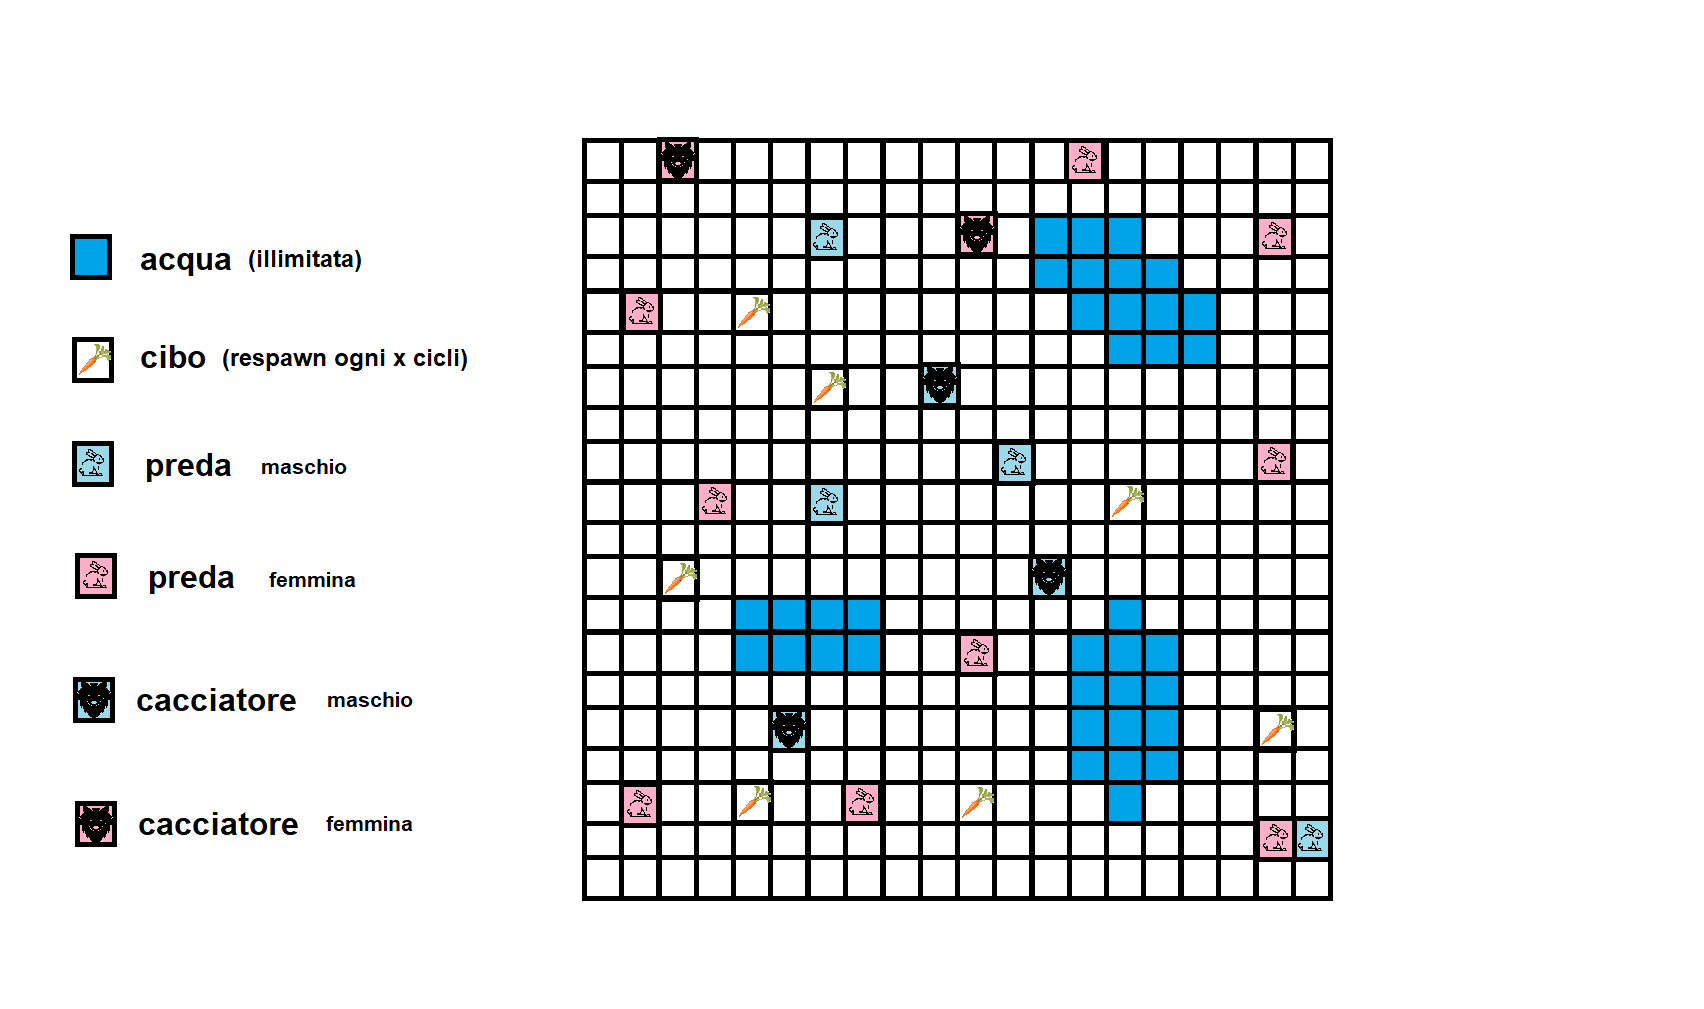
\includegraphics[scale = 0.4]{mockup.png}
    \label{fig1}
    \caption{Mockup in scala dell'ambiente e degli agenti al suo interno.}
\end{figure}

\newpage

Di seguito la documentazione (compresi due video) di riferimento fino ad ora reperita e la relativa bibliografia: 
\begin{itemize}
    \item Modello netlogo \cite{NetLogoModel} 
    \item  Lotka \cite{Lotka}
    \item Volterra \cite{Volterra}
    \item Physics of Risks \cite{PhysicsofRisk}
    \item Wilensky \cite{Wilensky}
    \item video youtube: Simulating an ecosystem \cite{YTVideo1}
    
     \item video youtube: Natural selection \cite{YTVideo2}
\end{itemize}


\medskip
\printbibliography	



\end{document}
